\documentclass[IJ]{cesj}
\usepackage{graphicx}
\usepackage{listings}

\author{Ga\"etan Lehmann}
\institute{Biologie du d\'eveloppement et de la reproduction, INRA de Jouy-en-Josas}

\title{InvertIntensityImageFilter}
\abstract{InvertIntensityImageFilter is a convenient filter to invert the intensity of an image.}
\keyword{UnaryFunctorImageFilter}
\year{2005}

\leftmark{Ga\"etan Lehmann}
\rightmark{Ga\"etan Lehmann}

\begin{document}
\lstset{language=c++}
\maketitle
% \tableofcontents

\section{Description}
InvertIntensityImageFilter is a convenient filter to invert the intensity of an image. An image can already be inverted with ITK, but it requires to use a more complex filter (ShiftScaleImageFilter or IntensityWindowingImageFilter).

\section{Implementation}
InvertIntensityImageFilter is based on UnaryFunctorImageFilter and simply subtract the maximum value to all pixels before casting the result to the output pixel type.
\begin{lstlisting}
TOutput result = static_cast<TOutput>( m_Maximum - x );
\end{lstlisting}
The maximum value is not computed by the filter to avoid iterating twice over the input image. It may be given by the user, but the default value (NumericTraits$<$ InputPixelType $>$::max()) must be correct in most of cases.
 
\section{Performances}
The performances of the different solutions have been measured on a linux box with an Athlon64 2800+ and repeated 100 fold. The inverted image is an 8 bits 3D image of size 371x371x34\footnote{Image of ES cells from mima2 (http://mima2.jouy.inra.fr/)}. Results are reported in Table~\ref{perf}.

\begin{table}
\centering
\begin{tabular}{cc}
\hline
filter & Execution time \\
\hline
\hline
InvertIntensityImageFilter & 0.0367 s \\
ShiftScaleImageFilter & 0.0842 s \\
IntensityWindowingImageFilter & 0.0876 s \\
\hline
\end{tabular}
\caption{Execution time.\label{perf}}
\end{table}


\section{Usage}
As usual, user has to include the header:
\begin{lstlisting}
#include "itkInvertIntensityImageFilter.h"
\end{lstlisting}
and declare the type, instanciate the filter, and set the input image
\begin{lstlisting}
typedef itk::InvertIntensityImageFilter< InputType, OuputType >
  InvertType;
InvertType::Pointer invert = InvertType::New();
invert->SetInput( filter->GetOutput() );
\end{lstlisting}
The maximum value can be set with the SetMaximum() method, and read with GetMaximum().
\begin{lstlisting}
invert->SetMaximum( 80 );
\end{lstlisting}
The default is itk::NumericTraits$<$ PType $>$::max().

\section{Example}
This filter can be use to invert a binary image, a distance map, etc.

\begin{figure}
\centering
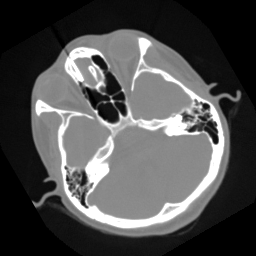
\includegraphics[width=0.5\textwidth]{cthead1}
\caption{The input image.}
\end{figure}

\begin{figure}
\centering
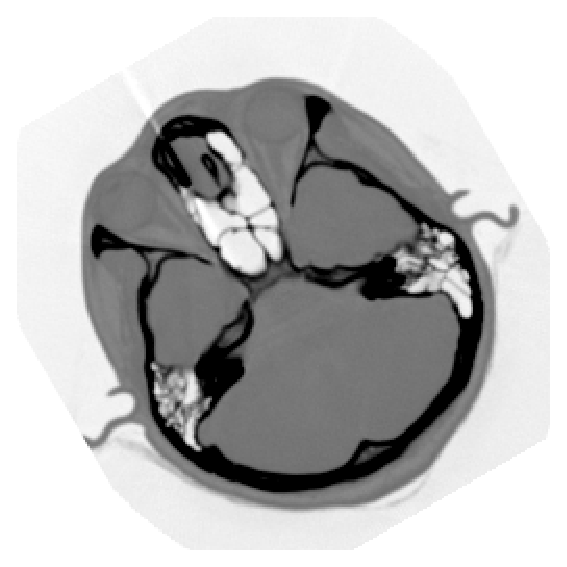
\includegraphics[width=0.5\textwidth]{invert}
\caption{The inverted image.}
\end{figure}

\end{document}
